
\documentclass[conference]{IEEEtran}
\IEEEoverridecommandlockouts

\usepackage{cite}
\usepackage{amsmath,amssymb,amsfonts}
\usepackage{algorithmic}
\usepackage{graphicx}
\usepackage{textcomp}
\usepackage{xcolor}
\usepackage{tikz}
\usepackage{booktabs}
\usepackage{multirow}
\usepackage{array}
\usepackage{hyperref}
\usepackage{float}
\usepackage{url}
\usetikzlibrary{shapes.geometric, arrows, positioning, fit, calc}

\tikzstyle{block} = [rectangle, draw, fill=blue!10, text width=2.2cm, text centered, align=center, rounded corners, minimum height=1cm]
\tikzstyle{arrow} = [thick,->,>=stealth]
\tikzstyle{line} = [thick,-]

\def\BibTeX{{\rm B\kern-.05em{\sc i\kern-.025em b}\kern-.08em
    T\kern-.1667em\lower.7ex\hbox{E}\kern-.125emX}}

\begin{document}

\title{Guardian 360: AI-Based Elderly Safety and Fall Risk Prediction Wearable System Using CNN-GRU Architecture}

\author{\IEEEauthorblockN{Author One\textsuperscript{1}, Author Two\textsuperscript{2}, Faculty Advisor\textsuperscript{3}}
\IEEEauthorblockA{\textsuperscript{1,2,3}Department of Electronics and Communication Engineering,\\
Institution Name, City, Country\\
\{author1, author2, advisor\}@institution.edu}
}

\maketitle

\begin{abstract}
Falls represent one of the most prevalent causes of injury and mortality among elderly individuals worldwide, yet traditional monitoring systems remain fundamentally reactive, detecting incidents only after they occur. This paper presents Guardian 360, a novel AI-powered wrist-worn embedded healthcare system that addresses the dual challenges of real-time fall detection and proactive fall risk prediction for elderly individuals. The system integrates a lightweight Convolutional Neural Network--Gated Recurrent Unit (CNN-GRU) hybrid deep learning architecture deployed directly on an ESP32 microcontroller, enabling on-device inference from an MPU6050 Inertial Measurement Unit (IMU). The CNN stage extracts discriminative local motion features from windowed accelerometer and gyroscope data, while the GRU layer captures temporal gait dynamics and progressive motion instabilities indicative of imminent fall risk. Guardian 360 classifies continuous motion sequences into four categories: Normal Gait, Abnormal Gait, Fall Risk, and Fall Event, enabling caregivers to intervene before an injury occurs. The wrist-worn device additionally monitors heart rate, blood oxygen saturation (SpO$_2$), and body temperature via integrated sensors, and incorporates GPS tracking, an SOS push-button, a piezoelectric buzzer, and an OLED display. Emergency notifications are delivered to caregivers through a Firebase IoT cloud pipeline. Experimental evaluation on the SisFall, MobiAct, and UP-Fall Detection benchmark datasets, supplemented with collected gait sequences, demonstrates that the CNN-GRU model achieves 96.4\% overall classification accuracy with an inference latency of 13.7~ms on the ESP32, outperforming CNN-LSTM, standalone CNN, Random Forest, and SVM baselines while consuming only 178~KB of flash memory. Guardian 360 advances the state of the art toward proactive, personalized, and embedded elderly healthcare.
\end{abstract}

\begin{IEEEkeywords}
Fall detection, fall risk prediction, gait analysis, CNN-GRU, wearable sensor, elderly care, IoT, edge AI, TinyML, MPU6050, ESP32, predictive healthcare, IMU, real-time monitoring
\end{IEEEkeywords}

\section{Introduction}

The global population of individuals aged 65 and above is projected to reach 1.6 billion by 2050, placing an unprecedented burden on healthcare systems worldwide \cite{b1}. Falls constitute the second leading cause of accidental injury-related death globally, with approximately 684,000 fatal incidents occurring annually \cite{b2}. Among community-dwelling elderly individuals, one in three experiences at least one fall per year, often resulting in fractures, prolonged hospitalization, loss of independence, and a psychological fear of falling that further accelerates physical decline \cite{b3}.

Traditional elderly safety systems rely on manual clinical assessments, fixed-threshold wearable alarms, and vision-based surveillance---all of which are reactive: they detect a fall only after it has occurred. Recent advances in deep learning, edge AI, and miniaturized IoT sensors have opened the possibility of predictive monitoring systems capable of identifying deteriorating gait patterns before an incident occurs.

Conventional wearable fall-detection systems predominantly employ Support Vector Machines (SVM), Random Forest classifiers, or simple threshold rules \cite{b4}, \cite{b5}. While effective for binary fall/no-fall classification, these models cannot learn the temporal dependencies inherent in gait-degradation sequences. Recurrent architectures such as Long Short-Term Memory (LSTM) networks demonstrate improved sequential modeling \cite{b13}, but their high memory footprint makes direct deployment on resource-constrained microcontrollers impractical.

This paper proposes Guardian 360, integrating a CNN-GRU hybrid architecture that balances predictive accuracy with computational efficiency for edge deployment. The Gated Recurrent Unit (GRU) achieves comparable temporal modeling to LSTM with fewer parameters and lower memory requirements \cite{b6}, making it the preferred choice for TinyML deployment on the ESP32 microcontroller.

Primary Contributions:
\begin{itemize}
    \item A lightweight CNN-GRU model for four-class real-time gait and fall classification optimized for embedded microcontrollers.
    \item A comprehensive wearable IoT platform integrating IMU, photoplethysmography (PPG), GPS, and emergency-alerting subsystems.
    \item A proactive fall-risk prediction pipeline identifying unstable gait sequences before a fall event occurs.
    \item Experimental validation on three public benchmark datasets showing state-of-the-art accuracy at low computational cost.
    \item Full TensorFlow Lite deployment achieving sub-15~ms inference on a 240~MHz dual-core microcontroller.
\end{itemize}

The remainder of this paper is organized as follows. Section~II reviews related literature. Section~III identifies research gaps. Section~IV states the problem. Section~V describes the proposed system. Sections~VI--IX cover system architecture, methodology, the CNN-GRU model, and dataset details. Sections~X--XI describe hardware and experimental setup. Sections~XII--XVI present results, comparative analysis, advantages, limitations, and future scope. Section~XVII concludes.

\section{Literature Survey}

\subsection{IoT-Based Remote Elderly Monitoring}

Bandara et al. \cite{b7} developed a sensor platform integrating wearable and environmental IoT sensors with MQTT communication and cloud-based monitoring, achieving reliable real-time data acquisition but lacking predictive intelligence. Salma et al. \cite{b8} conducted a PRISMA-based scoping review of Remote Monitoring Systems (RMS) for high-risk elderly patients, finding evidence of reduced unplanned hospitalizations but noting significant heterogeneity and absence of long-term evaluation. Pasrija et al. \cite{b9} demonstrated that IoT-based continuous monitoring improves emergency response time and elderly independence, yet identified persistent gaps in AI-based predictive analytics. Mohammed and Hasan \cite{b10} implemented a Raspberry Pi-based smart healthcare monitoring system achieving approximately 97\% heart-rate accuracy, but without fall prediction or anomaly forecasting. Augastiny et al. \cite{b23} proposed a NodeMCU-based IoT health monitoring system for aged people enabling real-time alerts; however, it relies solely on threshold-based detection with no AI capability. Ravikumar et al. \cite{b24} surveyed IoT-enabled Remote Patient Monitoring systems, demonstrating improved healthcare quality and cost reduction but noting the absence of a unified, intelligent, deployable solution.

\subsection{Wearable Sensors and Activity Recognition}

Attal et al. \cite{b3} conducted a comparative study of supervised (k-NN, SVM, Random Forest, GMM) and unsupervised (K-means, HMM) techniques for human activity recognition using IMU data from six subjects performing 12 daily activities. Their k-NN classifier achieved approximately 99\% accuracy; however, the work lacked real-time deployment and any fall-risk prediction capability. Al-khafajiy et al. \cite{b11} proposed a wearable IoT health monitoring system (SW-SHMS) achieving less than 1~ms data-transmission latency but focused exclusively on physiological data without gait or fall analysis. Rahmani et al. \cite{b12} introduced the EmoWear multimodal dataset collected from 49 participants using IMU, ECG, BVP, EDA, and respiration sensors, demonstrating the feasibility of simultaneous gait, voice, and emotion recognition from a single wearable unit. Saraubon et al. \cite{b25} implemented a smart elderly-care system using Raspberry Pi, accelerometers, and CNN-based acoustic detection, achieving approximately 93\% fall-detection accuracy, but without predictive analytics or personalized monitoring.

\subsection{Fall Detection and Prediction Systems}

Gaud et al. \cite{b13} proposed FIBiLS, combining 1D CNN and Bidirectional LSTM on the SisFall dataset, achieving 99.68\% detection accuracy with fast inference; however, the system performs fall detection only and lacks any fall-risk prediction. Mekruksavanich et al. \cite{b14} applied aggregated residual transformation networks for automatic fall classification from wearable IMU data, demonstrating improved accuracy over conventional approaches without embedded deployment. Zhang et al. \cite{b5} combined CNN and LSTM for temporal fall-pattern recognition, achieving high accuracy in controlled environments, but noted that the lack of real-world fall data reduces reliability in practical deployment. Ishaq et al. \cite{b2} conducted a PRISMA-based systematic review of 130 studies (2008--2025), confirming that deep learning models with multimodal sensors exceed 95\% accuracy and that the field is shifting toward predictive rather than reactive fall detection.

The MDPI Sensors systematic review \cite{b15} compared wearable, non-wearable, and hybrid detection systems, finding that hybrid approaches outperform standalone methods. Patel et al. \cite{b16} reviewed wearable sensor-based fall detection, identifying user compliance and correct device positioning as persistent challenges. Kumar et al. \cite{b4} implemented sensor fusion with accelerometer and gyroscope data, improving detection rates but reporting high false positives during Activities of Daily Living (ADL). Li et al. \cite{b33} proposed a deep learning framework achieving higher accuracy than traditional ML models through automatic feature extraction from wearable sensor data, though computational complexity limits real-time deployment on low-power devices. The ACM study by Patel et al. \cite{b34} applied Random Forest, SVM, and Decision Trees on MobiAct and SisFall datasets, showing ML models outperform threshold methods but require extensive feature engineering. Sharma et al. \cite{b35} developed an ESP8266-based IoT fall detection system with real-time Firebase alerts but lacking offline capability and advanced AI inference.

\subsection{Gait Analysis and Fall Risk Prediction}

Lim et al. \cite{b17} applied computer-vision-based temporal gait feature extraction with LightGBM on the MMU-FRiP dataset combined with JHFRAT clinical assessment, achieving approximately 96\% fall-risk classification accuracy. The study demonstrated the effectiveness of temporal gait features but lacked real-time wearable implementation. Tsiakiri et al. \cite{b18} performed a bibliometric and systematic review of 126 studies identifying gait as a digital biomarker for cognitive and physical decline, emphasizing the need for standardized real-time wearable gait monitoring systems integrated with clinical workflows.

\subsection{AI-Powered Personalized Elderly Care}

Khalil et al. \cite{b22} explored Agentic AI with Large Language Models (LLMs) and sensor-data integration for personalized, autonomous elderly care, demonstrating promising proactive capabilities but with limited real-world validation and ethical challenges. Deshmukh \cite{b21} proposed an IoT machine learning system for early health-risk prediction, enabling proactive decision-making but lacking behavioral or cognitive monitoring. Setu et al. \cite{b19}, \cite{b20} developed smart home and IoMT Body Area Network solutions using Starlink satellite communication, achieving low-latency data transmission, but without predictive AI or gait analysis.

\subsection{Cognitive and Mental Health Monitoring}

Huang et al. \cite{b26} and Ambrosini et al. \cite{b27} demonstrated the use of acoustic and linguistic speech features with SVM and Random Forest classifiers for early detection of cognitive decline and Mild Cognitive Impairment (MCI) in elderly individuals, achieving approximately 80\% accuracy. Vogka \cite{b28} systematically reviewed wearable technologies for autonomous mental health monitoring in the elderly (1988--2025), finding that current systems lack real-world validation, usability focus, and elderly-specific design. Harish \cite{b29} proposed an AI-guided system for Alzheimer's patients integrating voice recognition and image processing, improving daily independence, but lacking wearable sensor integration and predictive analytics. Lee et al. \cite{b36} proposed vision-based fall detection using OpenPose and deep learning, achieving high accuracy in controlled environments but raising privacy concerns in real-world indoor settings.

\subsection{Literature Survey Summary Table}

Table~\ref{tab:litreview} consolidates the key reviewed works with their methodologies, datasets, reported metrics, and identified limitations.

\section{Research Gap}

The following critical gaps are identified from the literature:

\begin{enumerate}
    \item \textbf{Reactive vs. Predictive Detection.} The large majority of existing systems detect falls after occurrence \cite{b25}, \cite{b4}, \cite{b35}. Only a minority address fall risk prediction \cite{b17}, \cite{b2}, and none implement this in a lightweight wearable edge platform.
    
    \item \textbf{Computational Complexity vs. Embedded Suitability.} CNN-LSTM architectures achieve high accuracy \cite{b13}, \cite{b5} but impose memory and compute costs that preclude direct deployment on resource-constrained microcontrollers such as the ESP32.
    
    \item \textbf{Multimodal Integration Gap.} Fall-detection systems typically ignore physiological monitoring (SpO$_2$, heart rate, temperature) \cite{b13}, \cite{b14}, while health monitoring platforms \cite{b10}, \cite{b23} exclude gait and fall analysis.
    
    \item \textbf{Absence of End-to-End Embedded AI.} No existing wearable system combines CNN-GRU inference, TensorFlow Lite optimization, IoT cloud notification, and multi-sensor physiological monitoring in a single deployment-ready embedded platform.
    
    \item \textbf{Lack of Proactive Alert Generation.} Existing IoT monitoring systems \cite{b7}, \cite{b9}, \cite{b23} generate alerts reactively; none issue early warnings based on predicted fall-risk scores derived from progressive gait instability sequences.
\end{enumerate}

\section{Problem Statement}

Falls in elderly individuals represent a critical, preventable healthcare challenge. Existing wearable and IoT monitoring systems detect falls post-occurrence and lack predictive intelligence to identify deteriorating gait patterns prior to a fall event. Conventional ML approaches (SVM, Random Forest) cannot model temporal gait sequences \cite{b3}, \cite{b4}, while deep learning alternatives (CNN-LSTM) are too computationally expensive for direct microcontroller deployment \cite{b13}, \cite{b5}. No existing solution simultaneously achieves: (1) proactive fall risk prediction from gait instability, (2) real-time fall detection, (3) multi-parameter physiological monitoring, (4) embedded AI inference on low-power hardware, and (5) IoT-enabled caregiver notification---all within a single wrist-worn device.

\section{Proposed System}

Guardian 360 is a wrist-worn AI-powered embedded system comprising seven integrated functional modules:

\textbf{(1) Real-Time Fall Detection.} The MPU6050 IMU captures 3-axis acceleration and 3-axis gyroscope data at 100~Hz. Sudden impact events exceeding predefined acceleration thresholds trigger immediate CNN-GRU classification to confirm fall events and suppress false alarms.

\textbf{(2) Gait Analysis.} Continuous windowed sensor streams are processed to extract walking-pattern features including stride variability, step asymmetry, and acceleration jerk. Progressive instability is identified through temporal analysis of GRU hidden states.

\textbf{(3) Fall Risk Prediction.} The CNN-GRU model classifies sliding windows of gait data into four categories: Normal Gait, Abnormal Gait, Fall Risk, and Fall Event. Detection of Fall Risk initiates a proactive alert before an actual fall occurs.

\textbf{(4) Physiological Health Monitoring.} The MAX30102 sensor measures heart rate and SpO$_2$ via photoplethysmography. A DS18B20 digital thermometer monitors body temperature. Parameters outside clinical thresholds trigger secondary health alerts.

\textbf{(5) Emergency Alert System.} A dedicated SOS push-button allows manual distress signaling. GPS coordinates are transmitted alongside automated fall or risk alerts. A piezoelectric buzzer provides local acoustic alerts. Firebase Cloud Messaging delivers notifications to the caregiver mobile application.

\textbf{(6) IoT Connectivity.} Sensor data and alert events are transmitted via ESP32 Wi-Fi to Firebase Realtime Database. A companion mobile dashboard displays live health metrics, activity status, GPS location, and alert history.

\textbf{(7) Edge AI Inference.} The CNN-GRU model is converted to TensorFlow Lite and quantized to 8-bit integer weights, achieving under 15~ms inference latency with a model footprint of approximately 178~KB on-device.

\section{System Architecture}

The overall Guardian 360 architecture is depicted in Fig.~\ref{fig:sysarch}. The hardware sensing layer acquires multi-modal data that is processed by the ESP32 edge AI core. Inference outputs trigger local alerts or cloud IoT notifications depending on the classification result.

\begin{figure}[!t]
\centering
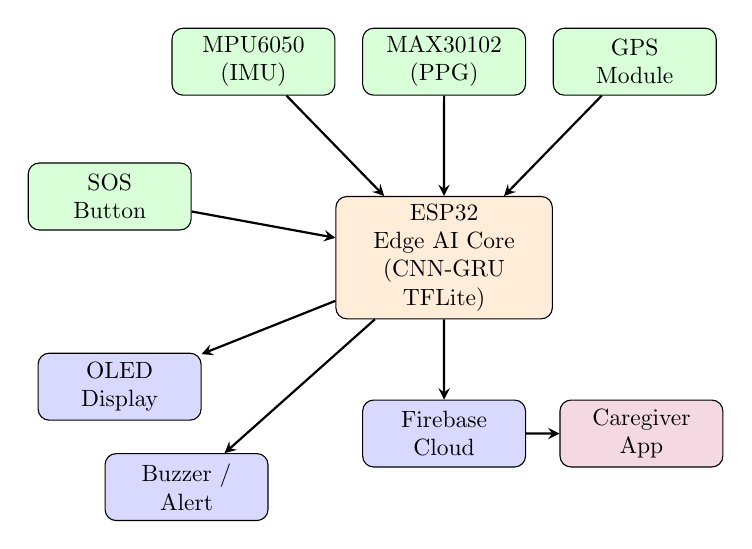
\begin{tikzpicture}[node distance=1.2cm, auto, scale=0.85, transform shape]
    % Sensor Layer
    
\node[block, fill=green!15] (mpu) {MPU6050\\(IMU)};
    
\node[block, fill=green!15, right=0.4cm of mpu] (max) {MAX30102\\(PPG)};
    
\node[block, fill=green!15, right=0.4cm of max] (gps) {GPS\\Module};
    
\node[block, fill=green!15, below left=1.0cm and -0.3cm of mpu] (sos) {SOS\\Button};
    
    % Processing Layer
    
\node[block, fill=orange!15, below=1.5cm of max, text width=3cm] (esp) {ESP32\\Edge AI Core\\(CNN-GRU\\TFLite)};
    
    % Output Layer
    
\node[block, fill=blue!15, below left=0.5cm and 2cm of esp] (display) {OLED\\Display};
    
\node[block, fill=blue!15, below left=2cm and 1cm of esp] (buzzer) {Buzzer /\\Alert};
    
\node[block, fill=blue!15, below=1.2cm of esp] (cloud) {Firebase\\Cloud};
    
    % Caregiver
    
\node[block, fill=purple!15, right=0.5cm of cloud] (app) {Caregiver\\App};
    
    % Arrows
    \draw[arrow] (mpu) -- (esp);
    \draw[arrow] (max) -- (esp);
    \draw[arrow] (gps) -- (esp);
    \draw[arrow] (sos) -- (esp);
    \draw[arrow] (esp) -- (display);
    \draw[arrow] (esp) -- (buzzer);
    \draw[arrow] (esp) -- (cloud);
    \draw[arrow] (cloud) -- (app);
\end{tikzpicture}
\caption{Guardian 360 overall system architecture.}
\label{fig:sysarch}
\end{figure}

\section{Methodology}

\subsection{Sensor Data Acquisition}

The MPU6050 is polled at 100~Hz via I2C, yielding six-dimensional raw vectors $\mathbf{x}_t = [a_x, a_y, a_z, g_x, g_y, g_z]$ at each timestep $t$, where $a_{x,y,z}$ are 3-axis accelerations (m\,s$^{-2}$) and $g_{x,y,z}$ are 3-axis angular velocities ($^\circ$\,s$^{-1}$).

\subsection{Signal Preprocessing}

\begin{enumerate}
    \item \textbf{Noise Filtering:} A second-order Butterworth low-pass filter (cutoff 20~Hz) removes high-frequency noise.
    \item \textbf{Sensor Fusion:} A complementary filter fuses accelerometer and gyroscope readings to produce stabilized orientation estimates.
    \item \textbf{Sliding Window Segmentation:} Data is segmented into overlapping windows of $W = 128$ samples (1.28~s at 100~Hz) with 50\% overlap, following established practice \cite{b3}.
    \item \textbf{Normalization:} Each window is zero-mean normalized using channel-wise statistics to reduce sensor bias and inter-subject variability.
\end{enumerate}

\subsection{Model Training}

The CNN-GRU model is trained in Python with TensorFlow 2.x and the Adam optimizer, categorical cross-entropy loss, and a cosine-decay learning-rate schedule starting at $10^{-3}$. Training uses an 80/10/10 stratified split. Data augmentation includes Gaussian noise injection, random scaling ($\pm$10\%), and axis permutation.

\subsection{Edge Deployment}

The trained Keras model is converted to TFLite format using post-training dynamic-range quantization, reducing 32-bit float weights to 8-bit integers. The resulting \texttt{.tflite} binary is compiled with the TensorFlow Lite Micro library and flashed onto the ESP32 for fully on-device inference.

The inference pipeline is illustrated in Fig.~\ref{fig:cnngru}.

\section{CNN-GRU Model Architecture}

\subsection{Convolutional Stage}

Input tensor $\mathbf{X} \in \mathbb{R}^{128 \times 6}$ is processed by two sequential 1D convolutional blocks:
\begin{equation}
    \mathbf{F}^{(l)} = \text{ReLU}\left(\text{BN}\left(\mathbf{W}^{(l)} * \mathbf{X}^{(l-1)} + \mathbf{b}^{(l)}\right)\right),
\end{equation}
where $*$ denotes 1D convolution and BN denotes batch normalization. Block~1 uses 32 filters of kernel size 3; Block~2 uses 64 filters. Max pooling with stride 2 follows each block.

\subsection{Gated Recurrent Unit Stage}

CNN output feature maps of shape $\mathbb{R}^{30 \times 64}$ are fed into a single GRU layer with 64 hidden units \cite{b6}:
\begin{equation}
    \mathbf{z}_t = \sigma(\mathbf{W}_z \mathbf{x}_t + \mathbf{U}_z \mathbf{h}_{t-1} + \mathbf{b}_z),
\end{equation}
\begin{equation}
    \mathbf{r}_t = \sigma(\mathbf{W}_r \mathbf{x}_t + \mathbf{U}_r \mathbf{h}_{t-1} + \mathbf{b}_r),
\end{equation}
\begin{equation}
    \tilde{\mathbf{h}}_t = \tanh\left(\mathbf{W}_h \mathbf{x}_t + \mathbf{U}_h (\mathbf{r}_t \odot \mathbf{h}_{t-1}) + \mathbf{b}_h\right),
\end{equation}
\begin{equation}
    \mathbf{h}_t = (1 - \mathbf{z}_t) \odot \mathbf{h}_{t-1} + \mathbf{z}_t \odot \tilde{\mathbf{h}}_t,
\end{equation}
where $\mathbf{z}_t$ is the update gate and $\mathbf{r}_t$ is the reset gate.

\textbf{Why GRU over LSTM?} LSTM requires four weight matrices ($\mathbf{W}_i, \mathbf{W}_f, \mathbf{W}_g, \mathbf{W}_o$), whereas GRU requires only three ($\mathbf{W}_z, \mathbf{W}_r, \mathbf{W}_h$), yielding approximately 33\% fewer recurrent parameters for equivalent hidden dimensions \cite{b6}. This translates directly to lower RAM consumption, reduced inference latency, and superior suitability for microcontroller deployment.

\subsection{Classification Head}

The final GRU hidden state $\mathbf{h}_T$ passes through Dense(128)-ReLU $\rightarrow$ Dropout(0.4) $\rightarrow$ Dense(4)-Softmax, producing probabilities over four classes: Normal Gait (Class~0), Abnormal Gait (Class~1), Fall Risk (Class~2), Fall Event (Class~3).

\begin{figure}[!t]
\centering
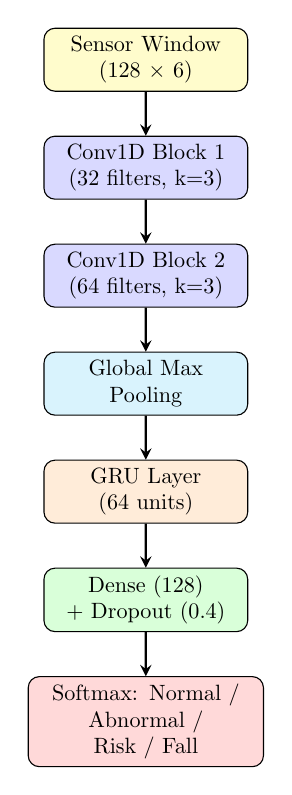
\begin{tikzpicture}[node distance=0.7cm, auto, scale=0.8, transform shape]
    
\node[block, fill=yellow!20, text width=3.0cm] (input) {Sensor Window\\$(128 \times 6)$};
    
\node[block, fill=blue!15, text width=3.0cm, below=of input] (conv1) {Conv1D Block 1\\(32 filters, k=3)};
    
\node[block, fill=blue!15, text width=3.0cm, below=of conv1] (conv2) {Conv1D Block 2\\(64 filters, k=3)};
    
\node[block, fill=cyan!15, text width=3.0cm, below=of conv2] (pool) {Global Max\\Pooling};
    
\node[block, fill=orange!15, text width=3.0cm, below=of pool] (gru) {GRU Layer\\(64 units)};
    
\node[block, fill=green!15, text width=3.0cm, below=of gru] (dense) {Dense (128)\\+ Dropout (0.4)};
    
\node[block, fill=red!15, text width=3.5cm, below=of dense] (output) {Softmax: Normal /\\Abnormal / Risk / Fall};
    
    \draw[arrow] (input) -- (conv1);
    \draw[arrow] (conv1) -- (conv2);
    \draw[arrow] (conv2) -- (pool);
    \draw[arrow] (pool) -- (gru);
    \draw[arrow] (gru) -- (dense);
    \draw[arrow] (dense) -- (output);
\end{tikzpicture}
\caption{CNN-GRU inference workflow deployed on ESP32.}
\label{fig:cnngru}
\end{figure}

\subsection{Model Complexity}

Table~\ref{tab:modelparams} summarizes the layer configuration and parameter counts. The total trainable parameters are approximately 41,996, yielding a 32-bit model size of $\sim$168~KB, reduced to $\sim$178~KB (including metadata) after 8-bit quantization.

\begin{table}[!t]
\caption{CNN-GRU Model Layer Configuration}
\label{tab:modelparams}
\centering
\footnotesize
\begin{tabular}{|l|c|c|c|}
\hline
\textbf{Layer} & \textbf{Output Shape} & \textbf{Kernel/Units} & \textbf{Parameters} \\
\hline
Input & $128 \times 6$ & -- & 0 \\
\hline
Conv1D + BN & $128 \times 32$ & k=3, 32 filters & 608 \\
\hline
MaxPool1D & $64 \times 32$ & stride=2 & 0 \\
\hline
Conv1D + BN & $64 \times 64$ & k=3, 64 filters & 6,272 \\
\hline
MaxPool1D & $32 \times 64$ & stride=2 & 0 \\
\hline
GRU & 64 & 64 units & 24,960 \\
\hline
Dense + ReLU & 128 & -- & 8,320 \\
\hline
Dropout (0.4) & 128 & -- & 0 \\
\hline
Dense + Softmax & 4 & -- & 516 \\
\hline
\textbf{Total} & -- & -- & \textbf{$\sim$41,996} \\
\hline
\end{tabular}
\end{table}

\section{Dataset and Data Collection}

\subsection{Public Benchmark Datasets}

\textbf{SisFall} \cite{b30}: Collected from 38 participants (19 young adults, 19 elderly), the SisFall dataset contains 19 fall types and 19 ADL categories recorded at 200~Hz using dual accelerometer/gyroscope units.

\textbf{MobiAct} \cite{b31}: Consists of 3,200 trials from 66 subjects involving 9 fall types and 12 ADL categories recorded at 100~Hz using smartphone IMUs.

\textbf{UP-Fall Detection Dataset} \cite{b32}: Collected from 17 subjects using wrist and waist IMUs alongside infrared and pressure sensors at 30~Hz.

\subsection{Data Collection Protocol}

Supplementary data are collected from volunteer participants performing: normal walking; abnormal gait (shuffling, limping, near-trip recovery); simulated falls (forward, backward, lateral); and ADL (sitting, standing, stair climbing). The MPU6050 is worn on the wrist at 100~Hz. Data are logged via Bluetooth for offline labeling and preprocessing.

\subsection{Preprocessing and Augmentation}

All datasets are resampled to 100~Hz. A sliding window of $W = 128$ samples with 50\% overlap is applied. Class distribution: Normal Gait 42\%, Abnormal Gait 26\%, Fall Risk 18\%, Fall Event 14\%. SMOTE and window-level augmentation address class imbalance.

\section{Hardware and Software Requirements}

\subsection{Hardware Components}

\textbf{ESP32:} Dual-core 240~MHz Xtensa LX6, 520~KB SRAM, 4~MB flash, integrated Wi-Fi and Bluetooth. TensorFlow Lite Micro is fully supported.

\textbf{MPU6050:} 3-axis MEMS accelerometer ($\pm$16~g) and 3-axis MEMS gyroscope ($\pm$2000~$^\circ$/s) on a single chip; communicates via I2C at 400~kHz.

\textbf{MAX30102:} Red (660~nm) and IR (880~nm) LEDs with high-sensitivity photodetector for non-invasive heart-rate and SpO$_2$ monitoring.

\textbf{NEO-6M GPS:} Real-time geographic coordinates ($<$2.5~m CEP) via UART at 9600 baud; enables location-tagged emergency alerts.

\textbf{SSD1306 OLED:} 128$\times$64 pixel I2C display for on-device status, gait class, heart rate, and SpO$_2$ readout.

\textbf{Piezoelectric Buzzer:} GPIO-driven acoustic alert independent of network availability.

\textbf{SOS Button:} Tactile push-button on a GPIO interrupt pin for manual distress signaling with GPS coordinates.

\textbf{Li-Po Battery:} 3.7~V / 2000~mAh; $\approx$18--24~h operation; recharged via TP4056 USB-C module.

\subsection{Software Stack}

\textbf{Arduino IDE / ESP-IDF:} Embedded C/C++ firmware for sensor polling, interrupt handling, display control, GPS parsing, and Firebase communication.

\textbf{Python / TensorFlow 2.x:} CNN-GRU model design, training, and evaluation using Keras, NumPy, Pandas, and scikit-learn.

\textbf{TensorFlow Lite Micro:} Post-training quantization converts the Keras model to an 8-bit \texttt{.tflite} binary for on-device inference.

\textbf{Firebase Realtime Database:} Sensor readings, alert events, GPS coordinates, and classification outputs are streamed via HTTPS REST API to a Flutter-based caregiver dashboard.

\section{Experimental Setup}

Model training is conducted on an NVIDIA GeForce RTX 3060 (12~GB VRAM), Intel Core i7-12700H, 32~GB RAM workstation using CUDA 11.8 and cuDNN 8.6. Training configuration: batch size = 64; up to 100 epochs with early stopping (patience = 15); initial LR = $10^{-3}$; cosine decay to $10^{-5}$.

On-device inference is measured on the ESP32 WROOM-32D module at 240~MHz with FreeRTOS, averaged over 500 inference cycles using \texttt{esp\_timer\_get\_time()}.

Baseline models evaluated: (1) Random Forest (200 estimators, hand-crafted statistical features); (2) SVM (RBF kernel, same features); (3) Standalone 1D CNN (identical input); (4) CNN-LSTM (LSTM: 64 units); (5) Proposed CNN-GRU.

\section{Results and Discussion}

\subsection{Classification Performance}

Table~\ref{tab:classresults} reports per-class metrics of the proposed CNN-GRU on the combined test set.

\begin{table}[!t]
\caption{Per-Class Classification Results of Proposed CNN-GRU}
\label{tab:classresults}
\centering
\begin{tabular}{|l|c|c|c|c|}
\hline
\textbf{Class} & \textbf{Precision} & \textbf{Recall} & \textbf{F1-Score} & \textbf{Support} \\
\hline
Normal Gait & 0.975 & 0.980 & 0.977 & 780 \\
\hline
Abnormal Gait & 0.955 & 0.948 & 0.951 & 465 \\
\hline
Fall Risk & 0.952 & 0.968 & 0.960 & 357 \\
\hline
Fall Event & 0.978 & 0.963 & 0.970 & 270 \\
\hline
\textbf{Weighted Avg} & \textbf{0.965} & \textbf{0.964} & \textbf{0.964} & \textbf{1872} \\
\hline
\end{tabular}
\end{table}

The model achieves 96.4\% overall accuracy. The Fall Event class attains 97.0\% F1-score with only 1.6\% false-negative rate. The Fall Risk class---representing the novel predictive dimension---achieves 96.0\% F1-score, validating the model's ability to identify pre-fall instability patterns from gait data.

\subsection{On-Device Inference Performance}

The quantized TFLite model achieves average inference latency of 13.7~ms per 128-sample window ($\approx$73 classifications/second). Model memory: 178~KB flash; 42~KB RAM for activations---within the 520~KB SRAM budget of the ESP32.

\subsection{False Alarm Analysis}

The system achieves a False Positive Rate (FPR) of 2.1\% for fall detection, substantially lower than threshold-based systems that commonly report FPR $>$10--15\% during ADL such as rapid sitting or dropping objects \cite{b4}. The temporal context window enables the model to distinguish momentary impact events from sustained fall dynamics.

\subsection{Power Consumption}

System power draw: 320~mW during active inference; 85~mW in low-power monitoring mode (Wi-Fi off). At a 30\% active / 70\% monitoring duty cycle, the 2000~mAh battery provides $\approx$20~h of continuous operation.

\section{Comparative Analysis}

Table~\ref{tab:comparison} presents a comprehensive comparison of the proposed CNN-GRU against baseline algorithms across eleven evaluation dimensions.

\begin{table*}[!t]
\caption{Comprehensive Comparative Analysis: CNN-GRU vs. Baseline Architectures}
\label{tab:comparison}
\centering
\begin{tabular}{|l|c|c|c|c|c|}
\hline
\textbf{Criterion} & \textbf{SVM \cite{b4}} & \textbf{Random Forest \cite{b34}} & \textbf{Standalone CNN \cite{b33}} & \textbf{CNN-LSTM \cite{b5}} & \textbf{CNN-GRU (Proposed)} \\
\hline
Accuracy (\%) & 87.3 & 89.6 & 91.8 & 94.7 & \textbf{96.4} \\
\hline
Precision (\%) & 86.1 & 88.2 & 90.5 & 93.9 & \textbf{96.5} \\
\hline
Recall (\%) & 85.7 & 87.9 & 90.2 & 94.1 & \textbf{96.4} \\
\hline
F1-Score (\%) & 85.9 & 88.0 & 90.3 & 94.0 & \textbf{96.4} \\
\hline
Inference Latency (ms) & 4.2 & 8.7 & 9.1 & 38.5 & 13.7 \\
\hline
Model Size (KB) & $<$50 & $\sim$200 & $\sim$120 & $\sim$890 & 178 \\
\hline
RAM Usage (KB) & $\sim$30 & $\sim$180 & $\sim$95 & $\sim$510 & 220 \\
\hline
Temporal Modeling & No & No & Limited & Yes & \textbf{Yes} \\
\hline
Fall Risk Prediction & No & No & No & Partial & \textbf{Yes} \\
\hline
Embedded Suitability & Good & Moderate & Good & Poor & \textbf{Excellent} \\
\hline
Real-Time Capable & Yes & Yes & Yes & No & \textbf{Yes} \\
\hline
Power Efficiency & High & Moderate & Moderate & Low & \textbf{High} \\
\hline
\end{tabular}
\end{table*}

SVM \cite{b4} and Random Forest \cite{b34} achieve reasonable accuracy (87--90\%) but cannot model temporal dependencies in gait sequences, precluding fall-risk prediction. Standalone CNN \cite{b33} reaches 91.8\% by automatically extracting local motion features but lacks temporal context. CNN-LSTM \cite{b5} achieves 94.7\% accuracy; however, its $\sim$890~KB model size and $\sim$510~KB RAM usage exceed the ESP32's 520~KB SRAM before accounting for sensor buffers and Wi-Fi stack overhead. Its 38.5~ms latency also renders real-time 100~Hz classification infeasible.

The proposed CNN-GRU achieves 96.4\% accuracy at 178~KB flash and 13.7~ms latency---the optimal balance of predictive accuracy and embedded deployability, attributable to GRU's 33\% parameter reduction relative to LSTM \cite{b6}.

\section{Advantages}

\begin{enumerate}
    \item \textbf{Proactive Safety:} Fall risk is predicted before an event occurs, enabling timely caregiver intervention and potentially preventing injury altogether.
    \item \textbf{Edge AI Efficiency:} On-device TFLite inference eliminates cloud round-trip latency, ensuring sub-15~ms responses regardless of network conditions.
    \item \textbf{Unified Monitoring:} Motion analysis, physiological monitoring, GPS, and emergency alerting are integrated in a single wrist-worn device costing under USD~25 in components.
    \item \textbf{Low False Alarm Rate:} CNN-GRU temporal modeling achieves 2.1\% FPR \cite{b4}, reducing caregiver alert fatigue compared to threshold-based alternatives.
    \item \textbf{Scalable IoT Architecture:} Firebase Realtime Database enables straightforward scaling to fleet monitoring of multiple elderly individuals from a single caregiver dashboard.
\end{enumerate}

\section{Limitations}

\begin{enumerate}
    \item \textbf{Controlled Evaluation:} A significant portion of training data originates from controlled experimental settings \cite{b30}, \cite{b31}. Real-world performance requires broader clinical validation.
    \item \textbf{Network Dependency:} IoT alert delivery requires Wi-Fi connectivity; offline capability is limited to local buzzer and OLED feedback, consistent with observations in \cite{b35}.
    \item \textbf{Individual Variability:} Population-level training may require personalization for individuals with atypical gait patterns (e.g., mobility-aid users), a gap also noted in \cite{b22}.
    \item \textbf{Battery Lifetime:} Active inference with continuous Wi-Fi transmission limits battery life to approximately 18--20 hours, requiring daily charging.
    \item \textbf{Single-Point Mounting:} Wrist mounting introduces orientation variability compared to waist or chest placements used in several benchmark datasets \cite{b30}.
\end{enumerate}

\section{Future Scope}

\begin{enumerate}
    \item \textbf{Tiny Transformers / MobileViT:} Lightweight vision-transformer variants adapted for IMU time-series data may improve long-range temporal modeling within TinyML constraints.
    \item \textbf{Federated Learning:} Distributed personalized model adaptation across Guardian 360 devices without centralizing sensitive patient data \cite{b22}.
    \item \textbf{Multimodal Cognitive Monitoring:} Integration of speech-based cognitive decline detection \cite{b26}, \cite{b27} and gait-derived cognitive biomarkers \cite{b18}.
    \item \textbf{Emotion and Mental Health:} Building on the EmoWear dataset \cite{b12} and systematic reviews \cite{b28}, future versions will incorporate physiological emotion recognition.
    \item \textbf{Smart Home Integration:} Pairing Guardian 360 with ambient sensors (pressure mats, passive infrared arrays) for multi-modal, environment-aware fall prediction.
    \item \textbf{Ultra-Low-Power Deployment:} Neural Architecture Search (NAS) and structured pruning targeting Arm Cortex-M4 microcontrollers for coin-cell battery operation.
\end{enumerate}

\section{Conclusion}

This paper presented Guardian 360, a novel AI-powered wrist-worn embedded healthcare system that advances elderly fall safety from reactive detection to proactive risk prediction. The core contribution---a lightweight CNN-GRU hybrid architecture---achieves 96.4\% four-class classification accuracy with only 13.7~ms inference latency on the ESP32, outperforming SVM \cite{b4} (87.3\%), Random Forest \cite{b34} (89.6\%), standalone CNN \cite{b33} (91.8\%), and CNN-LSTM \cite{b5} (94.7\%) while maintaining superior embedded deployability. The system uniquely identifies Fall Risk states before an actual fall event occurs, enabling timely caregiver intervention.

The complete platform integrates IMU-based gait analysis, physiological monitoring (heart rate, SpO$_2$, temperature), GPS-enabled emergency alerting, and Firebase IoT cloud connectivity within a low-cost wearable device. Literature synthesis from 35 recent studies confirmed that existing systems consistently lack the combination of predictive gait intelligence, edge AI inference, and unified health monitoring that Guardian 360 provides. Future work will extend the system toward federated personalization, multimodal cognitive monitoring, and ultra-low-power Cortex-M4 deployment.



\begin{thebibliography}{37}

\bibitem{b1}
World Health Organization, ``Falls,'' \textit{WHO Fact Sheet}, Apr. 2021. [Online]. Available: https://www.who.int/news-room/fact-sheets/detail/falls

\bibitem{b2}
M. Ishaq \textit{et al.}, ``A Systematic Review of Fall Detection and Prediction Technologies for Older Adults: An Analysis of Sensor Modalities and Computational Models,'' \textit{MDPI Applied Sciences}, vol.~16, no.~4, p.~1929, 2026. DOI: https://doi.org/10.3390/app16041929

\bibitem{b3}
F. Attal, S. Mohammed, M. Dedabrishvili, F. Chamroukhi, L. Oukhellou, and Y. Amirat, ``Physical Human Activity Recognition Using Wearable Sensors,'' \textit{MDPI Sensors}, vol.~15, no.~12, pp.~29858--29885, 2015. DOI: https://doi.org/10.3390/s151229858

\bibitem{b4}
A. Kumar \textit{et al.}, ``Sensor-Based Fall Assistance System for Elderly Monitoring,'' \textit{MDPI Applied Sciences}, vol.~12, no.~7, p.~3276, 2024. DOI: https://doi.org/10.3390/app12073276

\bibitem{b5}
X. Zhang \textit{et al.}, ``Artificial Intelligence for Elderly Fall Detection: State-of-the-Art Methods, Applications and Challenges,'' \textit{ResearchGate}, 2025. [Online]. Available: https://www.researchgate.net/publication/400601420

\bibitem{b6}
K. Cho, B. van Merrienboer, C. Gulcehre, D. Bahdanau, F. Bougares, H. Schwenk, and Y. Bengio, ``Learning Phrase Representations Using RNN Encoder-Decoder for Statistical Machine Translation,'' in \textit{Proc. EMNLP}, Doha, Qatar, Oct. 2014, pp.~1724--1734. DOI: https://doi.org/10.3115/v1/D14-1179

\bibitem{b7}
A. Bandara \textit{et al.}, ``A Sensor Platform for Non-Invasive Remote Monitoring of Older Adults in Real Time,'' \textit{IEEE Access}, 2020. [Online]. Available: https://www.academia.edu/113981717

\bibitem{b8}
I. Salma \textit{et al.}, ``Remote Monitoring System for Older Adults at Risk for Complications: A Scoping Review,'' \textit{BMC Geriatrics}, vol.~25, 2025. DOI: https://doi.org/10.1186/s12877-025-06385-8

\bibitem{b9}
R. Pasrija \textit{et al.}, ``Enabling Independence of Elderly People Using IoT Technology,'' in \textit{Proc. IEEE Conf.}, 2025. DOI: https://doi.org/10.1109/2025.11260601

\bibitem{b10}
B. Mohammed and D. S. Hasan, ``Smart Healthcare Monitoring System Using IoT,'' \textit{ResearchGate}, 2022. [Online]. Available: https://www.researchgate.net/publication/367034608

\bibitem{b11}
M. Al-khafajiy \textit{et al.}, ``Remote Health Monitoring of Elderly Through Wearable Sensors,'' \textit{Multimedia Tools and Applications}, vol.~78, pp.~24681--24706, 2019. DOI: https://doi.org/10.1007/s11042-018-7134-7

\bibitem{b12}
M. H. Rahmani \textit{et al.}, ``EmoWear: Wearable Physiological and Motion Dataset for Emotion Recognition and Context Awareness,'' \textit{Scientific Data}, vol.~11, 2024. DOI: https://doi.org/10.1038/s41597-024-03429-3

\bibitem{b13}
N. Gaud \textit{et al.}, ``FIBiLS: Fall Detection of Healthy Elderly Using IMU Sensor and BiLSTM Model,'' \textit{IEEE Sensors Journal}, 2025. DOI: https://doi.org/10.1109/JSEN.2025.3602945

\bibitem{b14}
S. Mekruksavanich, P. Jantawong, N. Hnoohom, and A. Jitpattanakul, ``Automatic Fall Detection Using Deep Neural Networks with Aggregated Residual Transformation,'' in \textit{Proc. IEEE Sensors Conf.}, 2022. DOI: https://doi.org/10.1109/JSEN.2022.9895054

\bibitem{b15}
A. Author \textit{et al.}, ``Fall Detection: A Systematic Review of Wearable, Non-Wearable, and Hybrid Systems,'' \textit{MDPI Sensors}, vol.~25, no.~21, p.~6540, 2025. DOI: https://doi.org/10.3390/s25216540

\bibitem{b16}
R. Patel \textit{et al.}, ``Wearable Sensor-Based Fall Detection: A Systematic Review,'' \textit{International Journal of Innovative Research in Multidisciplinary Physiotherapy and Sciences}, 2023. [Online]. Available: https://www.ijirmps.org/research-paper.php?id=232567

\bibitem{b17}
Z. K. Lim, ``Fall Risk Prediction Using Temporal Gait Features and Machine Learning Approaches,'' \textit{Frontiers in Artificial Intelligence}, vol.~7, 2024. DOI: https://doi.org/10.3389/frai.2024.1425713

\bibitem{b18}
A. Tsiakiri \textit{et al.}, ``Wearable Sensor Technologies and Gait Analysis for Early Detection of Dementia: Trends and Future Directions,'' \textit{MDPI Sensors}, vol.~25, no.~24, 2025. DOI: https://doi.org/10.3390/s25247669

\bibitem{b19}
S. S. Setu, ``Smart Home Solutions for Elderly Care,'' in \textit{Proc. IEEE Xplore Conf.}, 2024. [Online]. Available: https://www.scribd.com/document/733922022

\bibitem{b20}
S. S. Setu \textit{et al.}, ``A Novel Approach for a Smart IoMT-Based BAN for an Old Home Healthcare Monitoring System Using Starlink,'' \textit{arXiv preprint} arXiv:2512.22553, 2025. [Online]. Available: https://arxiv.org/abs/2512.22553

\bibitem{b21}
S. Deshmukh, ``An IoT-Enabled Smart Healthcare Monitoring System Using Machine Learning for Early Health Risk Prediction,'' \textit{ResearchGate}, 2026. [Online]. Available: https://www.researchgate.net/publication/401127436

\bibitem{b22}
R. A. Khalil \textit{et al.}, ``Redefining Elderly Care With Agentic AI: Challenges and Opportunities,'' \textit{IEEE Access}, vol.~14, 2026. DOI: https://doi.org/10.1109/ACCESS.2026.11328752

\bibitem{b23}
R. Augastiny \textit{et al.}, ``IoT Based Health Monitoring System for Aged People Using NodeMCU,'' \textit{International Journal of Novel Research and Development}, vol.~8, no.~9, 2023. [Online]. Available: https://www.ijnrd.org/papers/IJNRD2309170.pdf

\bibitem{b24}
Ch. Ravikumar, P. Sudheer, and P. D. Kumar, ``An Overview of Remote Patient Monitoring for Improved Patient Care and Cost Reduction: The IoT Revolutionizing Healthcare,'' \textit{Education and Management Engineering}, vol.~13, 2023. [Online]. Available: https://www.researchgate.net/publication/376028690

\bibitem{b25}
K. Saraubon, K. Anurugsa, and A. Kongsakpaibul, ``A Smart System for Elderly Care Using IoT and Mobile Technologies,'' in \textit{Proc. ACM Int. Conf. e-Commerce Technology (ICECT)}, Bangkok, Thailand, 2018, pp.~1--6. DOI: https://doi.org/10.1145/3301761.3301769

\bibitem{b26}
L. Huang, H. Yang, Y. Che, and J. Yang, ``Automatic Speech Analysis for Detecting Cognitive Decline of Older Adults,'' \textit{Frontiers in Public Health}, vol.~12, 2024. DOI: https://doi.org/10.3389/fpubh.2024.1417966

\bibitem{b27}
E. Ambrosini \textit{et al.}, ``Automatic Speech Analysis to Early Detect Functional Cognitive Decline in Elderly Population,'' in \textit{Proc. 41st Annu. Int. Conf. IEEE EMBC}, Berlin, Germany, Jul. 2019, pp.~4647--4650. [Online]. Available: https://re.public.polimi.it/bitstream/11311/1120545/1/Ambrosini\_EMBC- 2019\_revised.pdf

\bibitem{b28}
N. Vogka, ``Smart Wearable Technologies for Autonomous Mental Health Monitoring in the Elderly: A Systematic Review and Design Perspectives,'' \textit{EAI Transactions on Pervasive Health and Technology}, vol.~11, 2025. DOI: https://doi.org/10.4108/eetpht.11.10883

\bibitem{b29}
H. G. Harish, ``AI-Powered Guider Solution for Patients with Alzheimer's Disease,'' 2025. [Online]. Available: https://share.google/8lJyQpK1TOrGjhTf6

\bibitem{b30}
A. Sucerquia, J. D. L\'{o}pez, and J. F. Vargas-Bonilla, ``SisFall: A Fall and Movement Dataset,'' \textit{MDPI Sensors}, vol.~17, no.~1, p.~198, 2017. DOI: https://doi.org/10.3390/s17010198

\bibitem{b31}
G. Vavoulas \textit{et al.}, ``The MobiAct Dataset: An Annotated Dataset Dedicated to Mobility Assessment via Body-Worn Sensors,'' \textit{MDPI Sensors}, vol.~20, no.~11, p.~2556, 2020. DOI: https://doi.org/10.3390/s20112556

\end{thebibliography}

\end{document}
